\documentclass{beamer}
\let\vec\mathbf
\mode<presentation>
\usepackage{amsmath}
\usepackage{amssymb}
%\usepackage{advdate}
\usepackage{adjustbox}
%\usepackage{subcaption}
\usepackage{enumitem}
\usepackage{multicol}
\usepackage{mathtools}
\usepackage{listings}
\usepackage{url}
\usetheme{Boadilla}
\usecolortheme{lily}
\setbeamertemplate{footline}
{
  \leavevmode%
  \hbox{%
  \begin{beamercolorbox}[wd=\paperwidth,ht=2.25ex,dp=1ex,right]{author in head/foot}%
    \insertframenumber{} / \inserttotalframenumber\hspace*{2ex} 
  \end{beamercolorbox}}%
  \vskip0pt%
}
\setbeamertemplate{navigation symbols}{}
\providecommand{\nCr}[2]{\,^{#1}C_{#2}} % nCr
\providecommand{\nPr}[2]{\,^{#1}P_{#2}} % nPr
\providecommand{\mbf}{\mathbf}
\providecommand{\pr}[1]{\ensuremath{\Pr\left(#1\right)}}
\providecommand{\qfunc}[1]{\ensuremath{Q\left(#1\right)}}
\providecommand{\sbrak}[1]{\ensuremath{{}\left[#1\right]}}
\providecommand{\lsbrak}[1]{\ensuremath{{}\left[#1\right.}}
\providecommand{\rsbrak}[1]{\ensuremath{{}\left.#1\right]}}
\providecommand{\brak}[1]{\ensuremath{\left(#1\right)}}
\providecommand{\lbrak}[1]{\ensuremath{\left(#1\right.}}
\providecommand{\rbrak}[1]{\ensuremath{\left.#1\right)}}
\providecommand{\cbrak}[1]{\ensuremath{\left\{#1\right\}}}
\providecommand{\lcbrak}[1]{\ensuremath{\left\{#1\right.}}
\providecommand{\rcbrak}[1]{\ensuremath{\left.#1\right\}}}
\theoremstyle{remark}
\newtheorem{rem}{Remark}
\newcommand{\sgn}{\mathop{\mathrm{sgn}}}

\providecommand{\res}[1]{\Res\displaylimits_{#1}} 
\providecommand{\norm}[1]{\lVert#1\rVert}
\providecommand{\mtx}[1]{\mathbf{#1}}

\providecommand{\fourier}{\overset{\mathcal{F}}{ \rightleftharpoons}}
%\providecommand{\hilbert}{\overset{\mathcal{H}}{ \rightleftharpoons}}
\providecommand{\system}{\overset{\mathcal{H}}{ \longleftrightarrow}}
	%\newcommand{\solution}[2]{\textbf{Solution:}{#1}}
%\newcommand{\solution}{\noindent \textbf{Solution: }}
\providecommand{\dec}[2]{\ensuremath{\overset{#1}{\underset{#2}{\gtrless}}}}
\newcommand{\myvec}[1]{\ensuremath{\begin{pmatrix}#1\end{pmatrix}}}

\title{Matrices in Geometry - 1.9.24}
\author{EE25BTECH11035  Kushal B N}
\date{Aug, 2025}

\begin{document}

\maketitle


\begin{frame}
\tableofcontents
\end{frame}

\section{Problem Statement}
\begin{frame}
\frametitle{Problem Statement}
The x-coordinate of a point $\vec{P}$ is twice is y-coordinate. If $\vec{P}$ is equidistant from the points $\vec{Q}$$\brak{2,-5}$ and $\vec{R}$$\brak{-3,6}$, find the coordiantes of $\vec{P}$.
\end{frame}

\section{Solution}
\begin{frame}{Solution}
   Given $\vec{P}$$\myvec{2k\\k}$, $\vec{Q}\myvec{2\\-5}$, $\vec{R}\myvec{-3\\6}$.\\
   Distances $PQ$ = $PR$ \\
   So their norms must be equal and also the square of their norms.
   \begin{equation}
	   {\norm{\vec{Q}-\vec{P}}}^{2} = {\norm{\vec{R}-\vec{P}}}^2
   \end{equation}

\begin{equation}
    {\norm{\vec{P}}}^2 - 2\vec{P}^{\top}\vec{Q} + {\norm{\vec{Q}}}^2 = {\norm{\vec{P}}}^2 - 2\vec{P}^{\top}\vec{R} + {\norm{\vec{R}}}^2
\end{equation}

\begin{equation}
    \implies \frac{{\norm{\vec{Q}}}^2 - {\norm{\vec{R}}}^2}{2} = \vec{P}^{\top}\brak{\vec{Q}-\vec{R}}
\end{equation}
    
\end{frame}



\begin{frame}{Solution}
\begin{equation}
    {\norm{\vec{Q}}}^2 = \myvec{2&-5}\myvec{2\\-5} = 4+25 = 29
\end{equation}

\begin{equation}
    {\norm{\vec{R}}}^2 = \myvec{-3&6}\myvec{-3\\6} = 9+36 = 45
\end{equation}

\begin{equation}
    \vec{Q} - \vec{R} = \myvec{5\\-11}
\end{equation}

\begin{equation}
    \implies -8 = \myvec{2k&k}\myvec{5\\-11}
\end{equation}

\begin{equation}
    -8 = 10k - 11k = -k
\end{equation}

\begin{equation}
    \implies \fbox{k = 8}
\end{equation}

\end{frame}

\section{Final Answer}
\begin{frame}{Final Answer}
\begin{equation*}
    \fbox{k = 8}
\end{equation*}
	The coordinates of point P = $\myvec{16\\8}$.

\begin{figure}
    \centering
    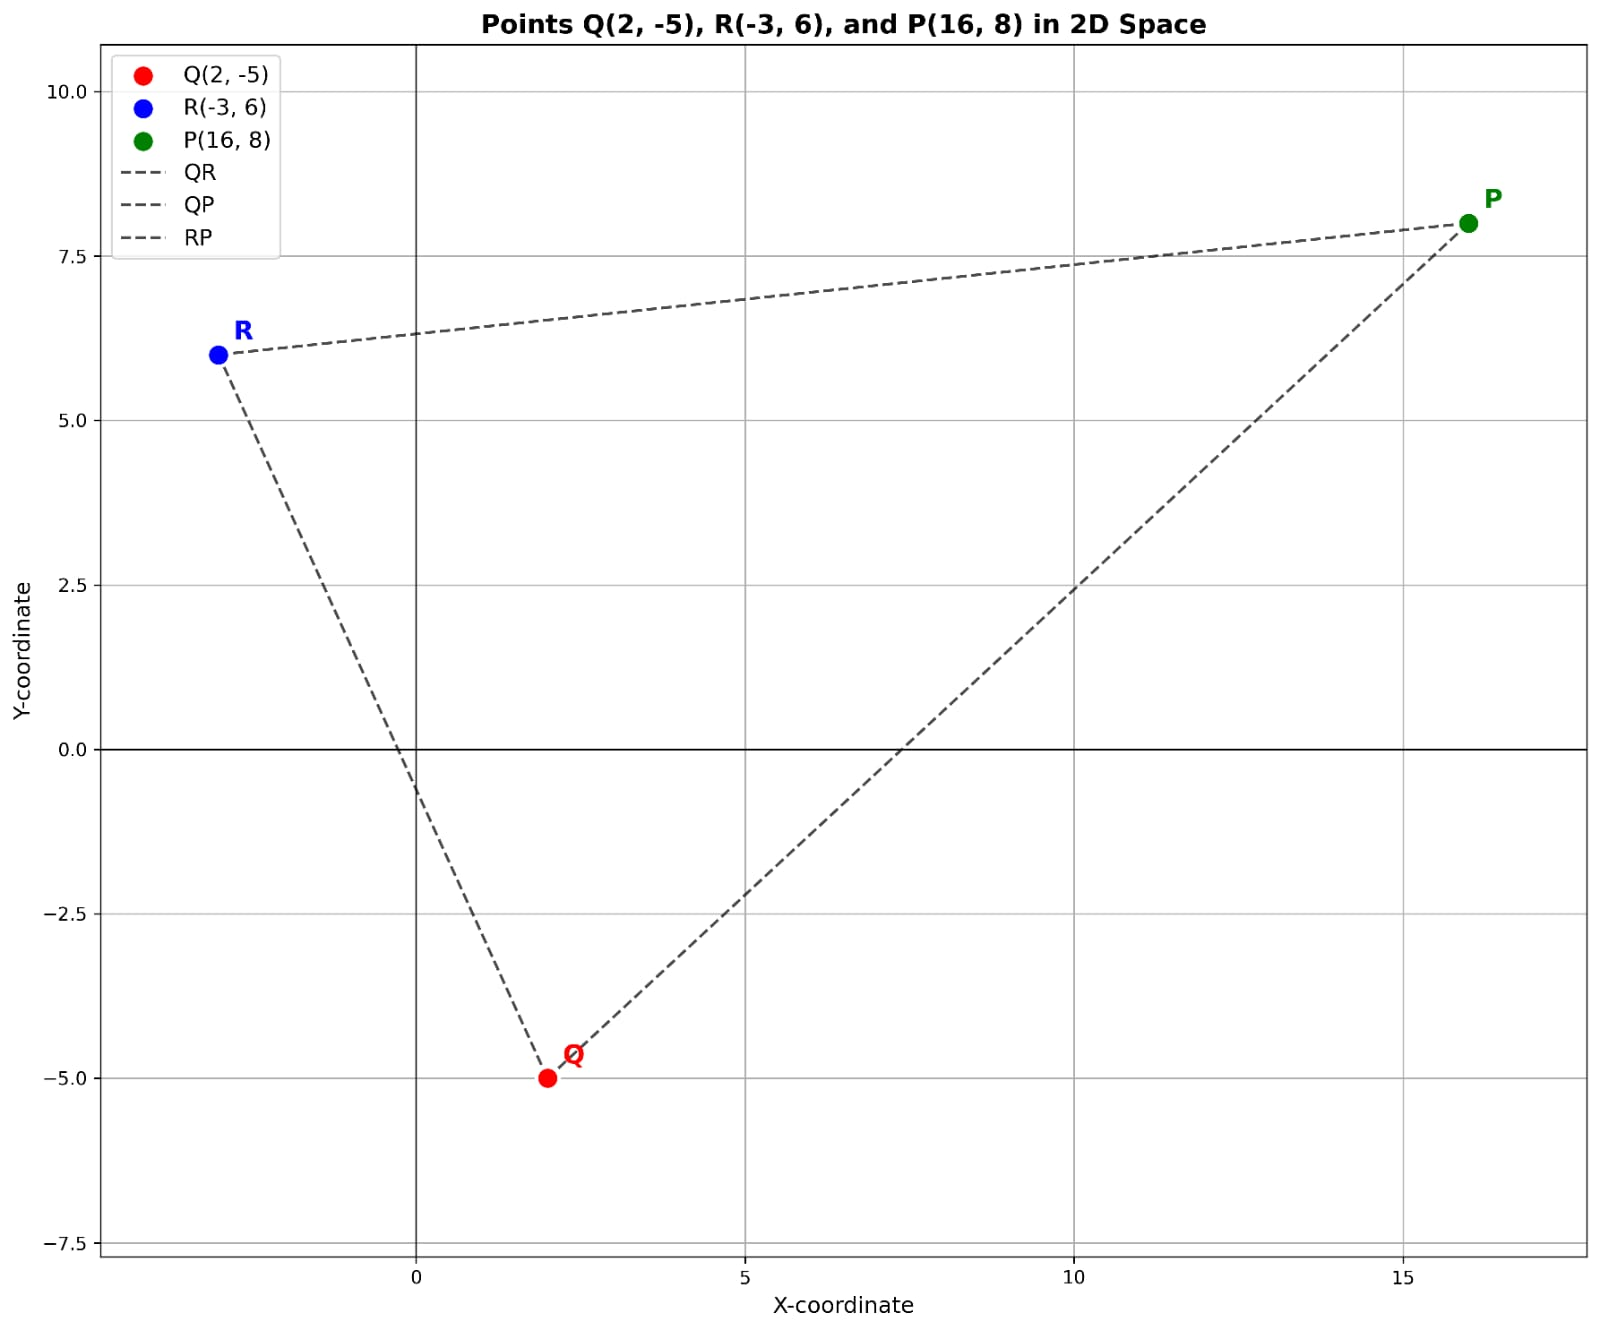
\includegraphics[width=0.5\linewidth]{figs/1.jpg}
\end{figure}

\end{frame}
\end{document}
